\documentclass[aspectratio=169]{beamer}

% Theme and appearance
\usetheme{Madrid}
\usecolortheme{default}

% Required packages
\usepackage{tikz}
\usepackage{pgfplots}
\usepackage{amsmath}
\usepackage{amsfonts}
\usepackage{amssymb}
\usepackage{graphicx}
\usepackage{booktabs}
\usepackage{array}
\usepackage{xcolor}

% TikZ libraries
\usetikzlibrary{shapes,arrows,positioning,calc,decorations.pathreplacing}
\usetikzlibrary{backgrounds,fit,shadows}

% Custom colors
\definecolor{networkblue}{RGB}{30,144,255}
\definecolor{networkgreen}{RGB}{34,139,34}
\definecolor{networkred}{RGB}{220,20,60}

% Title information
\title{Chapter 1: Introduction to Networks}
\author{Brendan Shea, PhD}
\institute{Introduction to Networking}
\date{2026}


\begin{document}
	
	% Slide 1: Title Slide
	\begin{frame}
		\titlepage
	\end{frame}
	
	% Slide 2: Learning Objectives and Exam Coverage
	\begin{frame}{Learning Objectives and Exam Coverage}
		\begin{itemize}
			\item Students will understand fundamental networking concepts and terminology used in modern computer networks.
			\item Students will be able to compare and contrast different network topologies and their appropriate use cases.
			\item Students will identify various network types including LANs, WANs, MANs, and specialized networks.
			\item Students will analyze network architectures and traffic flow patterns in enterprise environments.
		\end{itemize}
		
		\begin{alertblock}{CompTIA Network+ Exam Objective}
			Domain 1.0 Networking Concepts - 1.6: Compare and contrast network topologies, architectures, and types including mesh, hybrid, star/hub-and-spoke, spine-leaf, point-to-point, three-tier hierarchical model, and traffic flows.
		\end{alertblock}
	\end{frame}
	
	% Slide 3: What is a Network? - Basic Definition
	\begin{frame}{What is a Network? - Basic Definition}
		\begin{itemize}
			\item A \textbf{network} is defined as "a group or system of interconnected people or things."
			\item In computing, a network means two or more connected computers that can share resources.
			\item \textbf{Resources} include data, applications, office machines, Internet connections, or combinations thereof.
			\item Networks enable communication between devices using \textbf{binary code} consisting of 1s and 0s in specific patterns.
		\end{itemize}
		
		\begin{center}
			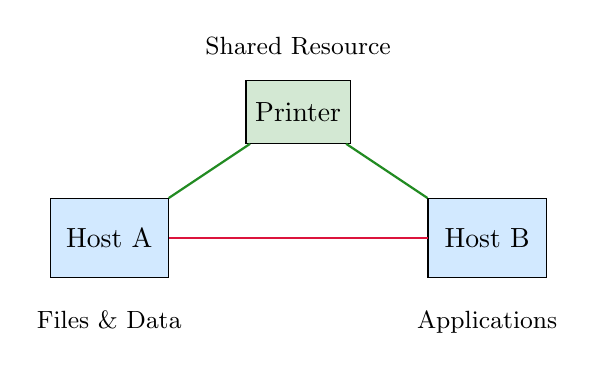
\begin{tikzpicture}[scale=0.8]
				% Draw two computers
				\node[draw, rectangle, fill=networkblue!20, minimum width=1.5cm, minimum height=1cm] (comp1) at (0,0) {Host A};
				\node[draw, rectangle, fill=networkblue!20, minimum width=1.5cm, minimum height=1cm] (comp2) at (6,0) {Host B};
				
				% Draw printer
				\node[draw, rectangle, fill=networkgreen!20, minimum width=1cm, minimum height=0.8cm] (printer) at (3,2) {Printer};
				
				% Draw connections
				\draw[thick, networkred] (comp1) -- (comp2);
				\draw[thick, networkgreen] (comp1) -- (printer);
				\draw[thick, networkgreen] (comp2) -- (printer);
				
				% Add labels
				\node[below=0.3cm of comp1] {\small Files \& Data};
				\node[below=0.3cm of comp2] {\small Applications};
				\node[above=0.2cm of printer] {\small Shared Resource};
			\end{tikzpicture}
		\end{center}
	\end{frame}
	
	% Slide 4: The Local Area Network (LAN) - Definition and Scope
	\begin{frame}{The Local Area Network (LAN) - Definition and Scope}
		\begin{itemize}
			\item A \textbf{Local Area Network (LAN)} is restricted to spanning a particular geographic location.
			\item Examples include office buildings, single departments, or home offices.
			\item Modern LANs have overcome historical limitations of 30 workstations and distance restrictions.
			\item \textbf{Workgroups} are logical zones that make administration easier by dividing large LANs.
		\end{itemize}
		
		\begin{exampleblock}{Scooby Doo Gang Network Example}
			The Mystery Inc. gang sets up their network in their headquarters building. Fred's computer in the main office needs to access files on Velma's computer in the research lab, and Shaggy's laptop in the kitchen needs to print investigation reports on the shared printer in Daphne's room. This entire building network represents their LAN.
		\end{exampleblock}
	\end{frame}
	
	% Slide 5: Common Network Components Overview
	\begin{frame}{Common Network Components Overview}
		\begin{itemize}
			\item Networks are composed of three main categories of devices that work together to enable communication.
			\item \textbf{Workstations} are powerful computers that provide resources to other users on the network.
			\item \textbf{Servers} are specialized computers running network operating systems to maintain and control networks.
			\item \textbf{Hosts} refer to any network device with an IP address in TCP/IP terminology.
		\end{itemize}
		
		\begin{block}{Key Distinction}
			The terms workstation, client, and host are often used interchangeably in casual conversation, but they have technical differences. A \textbf{client machine} is any device that can request access to resources from servers or workstations.
		\end{block}
	\end{frame}
	
	% Slide 6: Workstations vs. Clients - Understanding the Difference
	\begin{frame}{Workstations vs. Clients - Understanding the Difference}
		\begin{itemize}
			\item \textbf{Workstations} are powerful computers with multiple CPUs whose resources are available to network users.
			\item Workstations are often employed as systems that end users operate on a daily basis.
			\item \textbf{Client machines} are any devices that can request access to resources like printers or other hosts.
			\item The distinction matters technically, though people often use these terms interchangeably in practice.
		\end{itemize}
		
		\begin{exampleblock}{Scooby Doo Gang Example}
			Velma's high-powered computer with dual processors serves as a workstation, running complex analysis software while sharing its computational resources with the team. Meanwhile, Shaggy's basic laptop acts as a client machine, requesting access to files stored on Velma's workstation and sending print jobs to the shared printer.
		\end{exampleblock}
	\end{frame}
	
	% Slide 7: Server Types and Their Functions
	\begin{frame}{Server Types and Their Functions}
		\begin{itemize}
			\item \textbf{Servers} get their name because they are "at the service" of the network users.
			\item Servers run specialized \textbf{network operating systems} to maintain and control network operations.
			\item Dedicated servers optimize performance by handling one specific labor-intensive job.
			\item Servers require superior CPUs, hard-drive space, and memory compared to client machines.
		\end{itemize}
		
		\begin{center}
			\begin{tabular}{ll}
				\toprule
				\textbf{Server Type} & \textbf{Function} \\
				\midrule
				File Server & Stores and dispenses files \\
				Mail Server & Handles email functions \\
				Print Server & Manages network printers \\
				Web Server & Manages web content via HTTPS \\
				Application Server & Manages network applications \\
				Proxy Server & Handles tasks for other machines \\
				\bottomrule
			\end{tabular}
		\end{center}
	\end{frame}
	
	% Slide 8: Hosts - The TCP/IP Perspective
	\begin{frame}{Hosts - The TCP/IP Perspective}
		\begin{itemize}
			\item The term \textbf{host} can refer to almost any type of networking device in modern usage.
			\item In TCP/IP terminology, a host specifically means any network device with an IP address.
			\item The term originates from the era when only mainframes were considered intelligent network devices.
			\item Today, hosts include workstations, servers, routers, and any device that can communicate using TCP/IP.
		\end{itemize}
		
		\begin{alertblock}{Historical Context}
			In networking's "Jurassic period," mainframes were the only intelligent devices on networks and were called hosts. Everything else was considered "dumb terminals" without IP addresses. The term has evolved but retains its connection to devices capable of independent network communication.
		\end{alertblock}
	\end{frame}
	
	% Slide 9: Metropolitan Area Network (MAN)
	\begin{frame}{Metropolitan Area Network (MAN)}
		\begin{itemize}
			\item A \textbf{Metropolitan Area Network (MAN)} covers a metropolitan area to interconnect buildings and facilities.
			\item MANs typically operate over \textbf{carrier provider networks} using leased network connections.
			\item These networks can be thought of as concentrated WANs with high-speed interconnections.
			\item MANs often use in-ground fiber optics and provide cost-effective high-speed interconnects.
		\end{itemize}
		
		\begin{center}
			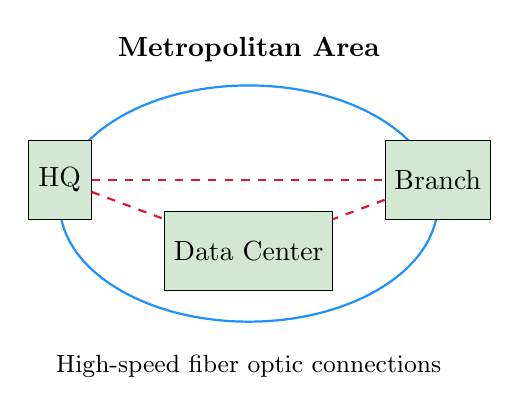
\begin{tikzpicture}[scale=0.6]
				% Draw city outline
				\draw[thick, networkblue] (0,0) ellipse (4cm and 2.5cm);
				\node[above] at (0,2.8) {\textbf{Metropolitan Area}};
				
				% Draw buildings
				\node[draw, rectangle, fill=networkgreen!20, minimum width=0.8cm, minimum height=1cm] (bldg1) at (-4,0.5) {HQ};
				\node[draw, rectangle, fill=networkgreen!20, minimum width=0.8cm, minimum height=1cm] (bldg2) at (4,0.5) {Branch};
				\node[draw, rectangle, fill=networkgreen!20, minimum width=0.8cm, minimum height=1cm] (bldg3) at (0,-1) {Data Center};
				
				% Draw fiber connections
				\draw[thick, networkred, dashed] (bldg1) -- (bldg2);
				\draw[thick, networkred, dashed] (bldg1) -- (bldg3);
				\draw[thick, networkred, dashed] (bldg2) -- (bldg3);
				
				\node[below] at (0,-3) {\small High-speed fiber optic connections};
			\end{tikzpicture}
		\end{center}
	\end{frame}
	
	% Slide 10: Wide Area Network (WAN) - Spanning the Distance
	\begin{frame}{Wide Area Network (WAN) - Spanning the Distance}
		\begin{itemize}
			\item A \textbf{Wide Area Network (WAN)} spans large geographic areas and links disparate locations.
			\item WANs usually employ routers and public links as defining criteria for their classification.
			\item The Internet is the largest example of a WAN, connecting networks worldwide.
			\item WANs can be \textbf{distributed} (interconnected computers in many places) or \textbf{centralized} (remote connections to a main location).
		\end{itemize}
		
		\begin{block}{Key WAN Characteristics}
			\begin{itemize}
				\item Usually need router ports for connectivity
				\item Span larger geographic areas than LANs
				\item Generally slower than LANs
				\item Allow selective connection timing and duration
				\item Can utilize private or public data transport media
			\end{itemize}
		\end{block}
	\end{frame}
	
	% Slide 11: Personal Area Network (PAN) - Close Proximity Connections
	\begin{frame}{Personal Area Network (PAN) - Close Proximity Connections}
		\begin{itemize}
			\item A \textbf{Personal Area Network (PAN)} enables close proximity connections between devices.
			\item PANs are commonly seen with smartphones and laptops in conference rooms for collaboration.
			\item While PANs can use wired connections like Ethernet or USB, wireless is more common.
			\item Typical wireless technologies include \textbf{Bluetooth}, \textbf{infrared}, and \textbf{ZigBee}.
		\end{itemize}
		
		\begin{exampleblock}{Scooby Doo Gang PAN Example}
			During a mystery investigation meeting, Fred uses Bluetooth to connect his smartphone to the conference room projector to display clues. Simultaneously, Velma's laptop connects to Daphne's tablet via Bluetooth to share forensic analysis data. These short-range connections (a few meters) form their PAN for the meeting.
		\end{exampleblock}
	\end{frame}
	
	% Slide 12: Campus Area Network (CAN)
	\begin{frame}{Campus Area Network (CAN)}
		\begin{itemize}
			\item A \textbf{Campus Area Network (CAN)} covers a limited geographical area such as a college or corporate campus.
			\item CANs typically interconnect LANs in various buildings and offer Wi-Fi components for roaming users.
			\item These networks are larger than LANs but smaller than MANs or WANs in scope.
			\item Most CANs provide Internet connectivity as well as access to data center resources.
		\end{itemize}
		
		\begin{center}
			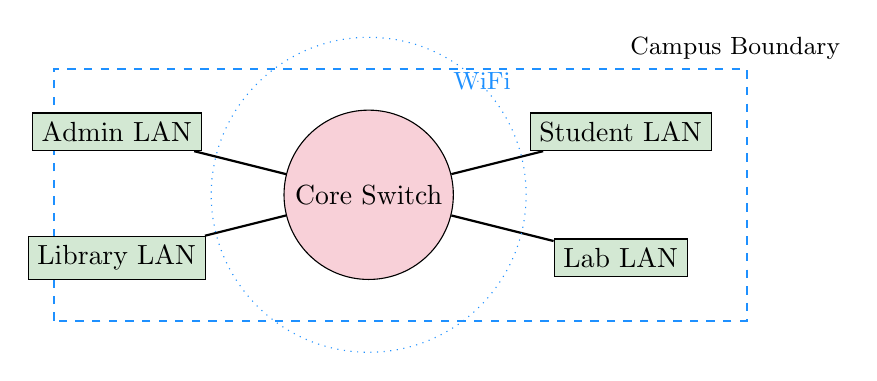
\begin{tikzpicture}[scale=0.8]
				% Draw campus boundary
				\draw[thick, networkblue, dashed] (-5,-2) rectangle (6,2);
				\node[above right] at (4,2) {\small Campus Boundary};
				
				% Draw buildings with LANs
				\node[draw, rectangle, fill=networkgreen!20] (admin) at (-4,1) {Admin LAN};
				\node[draw, rectangle, fill=networkgreen!20] (student) at (4,1) {Student LAN};
				\node[draw, rectangle, fill=networkgreen!20] (library) at (-4,-1) {Library LAN};
				\node[draw, rectangle, fill=networkgreen!20] (lab) at (4,-1) {Lab LAN};
				
				% Central switch
				\node[draw, circle, fill=networkred!20] (switch) at (0,0) {Core Switch};
				
				% Connections
				\draw[thick] (admin) -- (switch);
				\draw[thick] (student) -- (switch);
				\draw[thick] (library) -- (switch);
				\draw[thick] (lab) -- (switch);
				
				% WiFi coverage
				\draw[networkblue, dotted] (0,0) circle (2.5);
				\node[networkblue] at (1.8,1.8) {\small WiFi};
			\end{tikzpicture}
		\end{center}
		
		
	\end{frame}
	
	% Slide 17: Peer-to-Peer Networks - Decentralized Authority
	\begin{frame}{Peer-to-Peer Networks - Decentralized Authority}
		\begin{itemize}
			\item In \textbf{peer-to-peer networks}, computers have no central or special authority and are all equals.
			\item The authority to perform security checks lies with the computer that has the desired resource.
			\item Computers can simultaneously act as both client machines requesting resources and server machines providing resources.
			\item This architecture works well for small numbers of users with local backups and minimal security requirements.
		\end{itemize}
		
		\begin{alertblock}{Peer-to-Peer Challenges}
			Security presents major challenges because each user must maintain usernames and passwords on every machine. Passwords for the same user often change across different machines, creating a management nightmare. Backing up critical data becomes difficult without centralized storage.
		\end{alertblock}
	\end{frame}
	
	% Slide 18: Client-Server Networks - Centralized Management
	\begin{frame}{Client-Server Networks - Centralized Management}
		\begin{itemize}
			\item \textbf{Client-server networks} use a single server with a network operating system to manage the entire network.
			\item Client requests for resources go to the main server, which handles security and directs clients to desired resources.
			\item This architecture provides better organization because all files are stored in one centralized location.
			\item Security is tighter because all usernames and passwords are maintained on the dedicated server.
		\end{itemize}
		
		\begin{exampleblock}{Scooby Doo Gang Client-Server Example}
			Mystery Inc. sets up a client-server network where Velma's dedicated server computer stores all case files, clue databases, and monster identification records. When Fred needs to access witness statements from his laptop (client), he authenticates through Velma's server, which verifies his permissions and grants access to the appropriate files.
		\end{exampleblock}
	\end{frame}
	
	% Slide 19: Hybrid Network Architectures
	\begin{frame}{Hybrid Network Architectures}
		\begin{itemize}
			\item Many modern networks are a healthy blend of peer-to-peer and client-server architectures.
			\item \textbf{Hybrid networks} have specified servers while permitting simultaneous resource sharing from workstations.
			\item Supporting machines run server services reasonably well despite handling fewer inbound connections.
			\item Well-designed mixed environments benefit from the positive aspects of both architectural worlds.
		\end{itemize}
		
		\begin{center}
			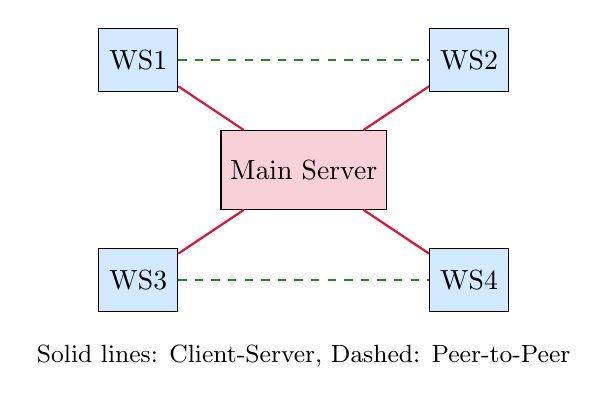
\begin{tikzpicture}[scale=0.7]
				% Draw central server
				\node[draw, rectangle, fill=networkred!20, minimum width=1.5cm, minimum height=1cm] (server) at (0,0) {Main Server};
				
				% Draw workstations that also share resources
				\node[draw, rectangle, fill=networkblue!20, minimum width=1cm, minimum height=0.8cm] (ws1) at (-3,2) {WS1};
				\node[draw, rectangle, fill=networkblue!20, minimum width=1cm, minimum height=0.8cm] (ws2) at (3,2) {WS2};
				\node[draw, rectangle, fill=networkblue!20, minimum width=1cm, minimum height=0.8cm] (ws3) at (-3,-2) {WS3};
				\node[draw, rectangle, fill=networkblue!20, minimum width=1cm, minimum height=0.8cm] (ws4) at (3,-2) {WS4};
				
				% Server connections (client-server)
				\draw[thick, networkred] (server) -- (ws1);
				\draw[thick, networkred] (server) -- (ws2);
				\draw[thick, networkred] (server) -- (ws3);
				\draw[thick, networkred] (server) -- (ws4);
				
				% Peer-to-peer connections
				\draw[thick, networkgreen, dashed] (ws1) -- (ws2);
				\draw[thick, networkgreen, dashed] (ws3) -- (ws4);
				
				\node[below] at (0,-3) {\small Solid lines: Client-Server, Dashed: Peer-to-Peer};
			\end{tikzpicture}
		\end{center}
	\end{frame}
	
	% Slide 20: Network Architecture Comparison
	\begin{frame}{Network Architecture Comparison}
		\begin{itemize}
			\item Network architecture choice depends on organization size, security needs, and administrative requirements.
			\item \textbf{Scalability} differs significantly between peer-to-peer and client-server implementations.
			\item Performance optimization varies based on centralized versus distributed resource management approaches.
			\item Cost considerations include both initial setup expenses and ongoing maintenance requirements.
		\end{itemize}
		
		\begin{center}
			\begin{tabular}{lcc}
				\toprule
				\textbf{Factor} & \textbf{Peer-to-Peer} & \textbf{Client-Server} \\
				\midrule
				Security & Decentralized & Centralized \\
				Scalability & Limited & Excellent \\
				Cost & Low initial & Higher initial \\
				Administration & Complex & Simplified \\
				Performance & Variable & Optimized \\
				Fault Tolerance & Distributed & Single point \\
				\bottomrule
			\end{tabular}
		\end{center}
	\end{frame}
	
	% Slide 21: Bus Topology - Linear Connections
	\begin{frame}{Bus Topology - Linear Connections}
		\begin{itemize}
			\item \textbf{Bus topology} is the most basic topology, consisting of two distinct and terminated ends.
			\item Each computer connects to one unbroken cable running the entire length of the network.
			\item Modern implementations use drop cables or "T" connectors instead of direct wire taps.
			\item All computers see all data flowing through the cable, but only the addressed computer receives it.
		\end{itemize}
		
		\begin{center}
			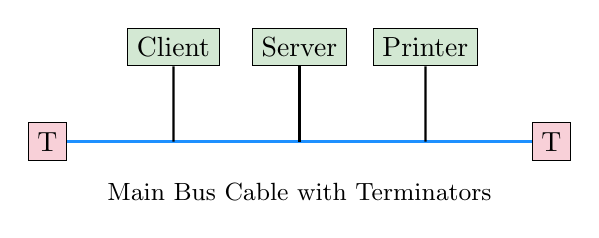
\begin{tikzpicture}[scale=0.8]
				% Draw main bus cable
				\draw[very thick, networkblue] (-4,0) -- (4,0);
				
				% Draw terminators
				\node[draw, rectangle, fill=networkred!20] at (-4,0) {T};
				\node[draw, rectangle, fill=networkred!20] at (4,0) {T};
				
				% Draw connected devices
				\node[draw, rectangle, fill=networkgreen!20] (client1) at (-2,1.5) {Client};
				\node[draw, rectangle, fill=networkgreen!20] (server) at (0,1.5) {Server};
				\node[draw, rectangle, fill=networkgreen!20] (printer) at (2,1.5) {Printer};
				
				% Draw drop cables
				\draw[thick] (-2,0) -- (client1);
				\draw[thick] (0,0) -- (server);
				\draw[thick] (2,0) -- (printer);
				
				\node[below] at (0,-0.5) {\small Main Bus Cable with Terminators};
			\end{tikzpicture}
		\end{center}
	\end{frame}
	
	% Slide 22: Star (Hub-and-Spoke) Topology
	\begin{frame}{Star (Hub-and-Spoke) Topology}
		\begin{itemize}
			\item \textbf{Star topology} connects computers to a central point with individual cables or wireless connections.
			\item The central device is typically a hub, switch, or access point managing all connections.
			\item Cable failure affects only the specific machine or segment, providing better fault tolerance.
			\item This topology offers excellent scalability by simply adding new cables to the central device.
		\end{itemize}
		
		\begin{center}
			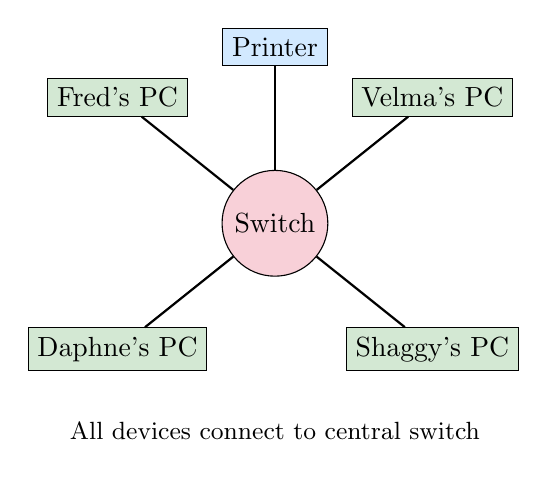
\begin{tikzpicture}[scale=0.8]
				% Draw central switch
				\node[draw, circle, fill=networkred!20, minimum size=1.2cm] (switch) at (0,0) {Switch};
				
				% Draw connected devices in star formation
				\node[draw, rectangle, fill=networkgreen!20] (pc1) at (-2.5,2) {Fred's PC};
				\node[draw, rectangle, fill=networkgreen!20] (pc2) at (2.5,2) {Velma's PC};
				\node[draw, rectangle, fill=networkgreen!20] (pc3) at (-2.5,-2) {Daphne's PC};
				\node[draw, rectangle, fill=networkgreen!20] (pc4) at (2.5,-2) {Shaggy's PC};
				\node[draw, rectangle, fill=networkblue!20] (printer) at (0,2.8) {Printer};
				
				% Draw connections
				\draw[thick] (switch) -- (pc1);
				\draw[thick] (switch) -- (pc2);
				\draw[thick] (switch) -- (pc3);
				\draw[thick] (switch) -- (pc4);
				\draw[thick] (switch) -- (printer);
				
				\node[below] at (0,-3) {\small All devices connect to central switch};
			\end{tikzpicture}
		\end{center}
	\end{frame}
	
	% Slide 23: Ring Topology - Circular Data Flow
	\begin{frame}{Ring Topology - Circular Data Flow}
		\begin{itemize}
			\item \textbf{Ring topology} connects each computer directly to other computers in a circular formation.
			\item Network data flows from computer to computer around the ring back to the source.
			\item Adding new devices requires breaking the cable ring, likely bringing down the entire network.
			\item This topology is expensive, difficult to reconfigure, and not fault-tolerant for LANs.
		\end{itemize}
		
		\begin{center}
			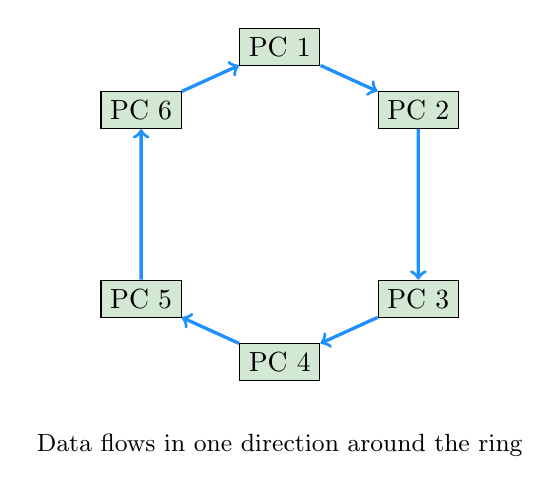
\begin{tikzpicture}[scale=0.8]
				% Draw ring with devices
				\node[draw, rectangle, fill=networkgreen!20] (pc1) at (0,2.5) {PC 1};
				\node[draw, rectangle, fill=networkgreen!20] (pc2) at (2.2,1.5) {PC 2};
				\node[draw, rectangle, fill=networkgreen!20] (pc3) at (2.2,-1.5) {PC 3};
				\node[draw, rectangle, fill=networkgreen!20] (pc4) at (0,-2.5) {PC 4};
				\node[draw, rectangle, fill=networkgreen!20] (pc5) at (-2.2,-1.5) {PC 5};
				\node[draw, rectangle, fill=networkgreen!20] (pc6) at (-2.2,1.5) {PC 6};
				
				% Draw ring connections with arrows showing direction
				\draw[very thick, networkblue, ->] (pc1) -- (pc2);
				\draw[very thick, networkblue, ->] (pc2) -- (pc3);
				\draw[very thick, networkblue, ->] (pc3) -- (pc4);
				\draw[very thick, networkblue, ->] (pc4) -- (pc5);
				\draw[very thick, networkblue, ->] (pc5) -- (pc6);
				\draw[very thick, networkblue, ->] (pc6) -- (pc1);
				
				\node[below] at (0,-3.5) {\small Data flows in one direction around the ring};
			\end{tikzpicture}
		\end{center}
	\end{frame}
	
	% Slide 24: Mesh Topology - Multiple Redundant Paths
	\begin{frame}{Mesh Topology - Multiple Redundant Paths}
		\begin{itemize}
			\item \textbf{Mesh topology} provides a path from every machine to every other machine in the network.
			\item Full mesh requires n(n-1)/2 connections, where n is the number of devices.
			\item \textbf{Partial mesh} provides some redundancy without connecting every device to every other device.
			\item This topology offers excellent fault tolerance but creates significant complexity and cost.
		\end{itemize}
		
		\begin{center}
			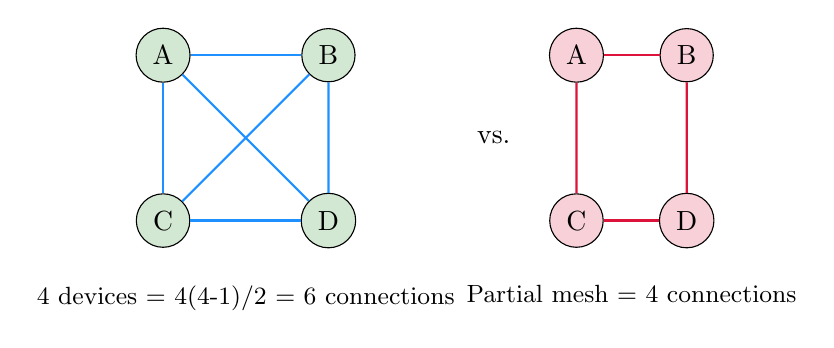
\begin{tikzpicture}[scale=0.7]
				% Draw four devices in full mesh
				\node[draw, circle, fill=networkgreen!20] (pc1) at (-1.5,1.5) {A};
				\node[draw, circle, fill=networkgreen!20] (pc2) at (1.5,1.5) {B};
				\node[draw, circle, fill=networkgreen!20] (pc3) at (-1.5,-1.5) {C};
				\node[draw, circle, fill=networkgreen!20] (pc4) at (1.5,-1.5) {D};
				
				% Draw all connections (full mesh)
				\draw[thick, networkblue] (pc1) -- (pc2);
				\draw[thick, networkblue] (pc1) -- (pc3);
				\draw[thick, networkblue] (pc1) -- (pc4);
				\draw[thick, networkblue] (pc2) -- (pc3);
				\draw[thick, networkblue] (pc2) -- (pc4);
				\draw[thick, networkblue] (pc3) -- (pc4);
				
				% Add calculation
				\node[below] at (0,-2.5) {\small 4 devices = 4(4-1)/2 = 6 connections};
				
				% Add partial mesh example
				\node at (4.5,0) {vs.};
				
				% Partial mesh with 4 devices
				\node[draw, circle, fill=networkred!20] (p1) at (6,1.5) {A};
				\node[draw, circle, fill=networkred!20] (p2) at (8,1.5) {B};
				\node[draw, circle, fill=networkred!20] (p3) at (6,-1.5) {C};
				\node[draw, circle, fill=networkred!20] (p4) at (8,-1.5) {D};
				
				% Partial connections
				\draw[thick, networkred] (p1) -- (p2);
				\draw[thick, networkred] (p1) -- (p3);
				\draw[thick, networkred] (p2) -- (p4);
				\draw[thick, networkred] (p3) -- (p4);
				
				\node[below] at (7,-2.5) {\small Partial mesh = 4 connections};
			\end{tikzpicture}
		\end{center}
	\end{frame}
	
	% Slide 25: Point-to-Point and Point-to-Multipoint Topologies
	\begin{frame}{Point-to-Point and Point-to-Multipoint Topologies}
		\begin{itemize}
			\item \textbf{Point-to-point topology} provides a direct connection between two routers or switches.
			\item This creates one communication path that can be physical (serial cable) or logical (circuit within Frame Relay/MPLS).
			\item \textbf{Point-to-multipoint topology} connects one interface on a router to multiple destination routers.
			\item All routers and interfaces in point-to-multipoint connections are part of the same network.
		\end{itemize}
		
		\begin{center}
			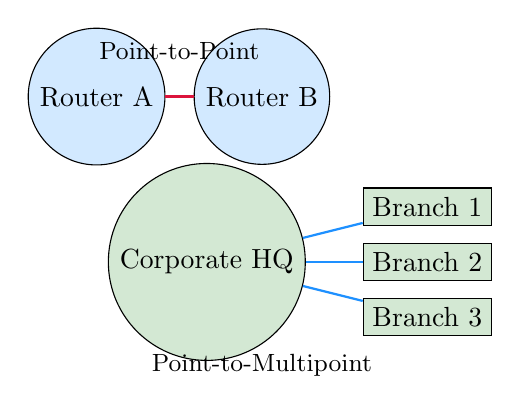
\begin{tikzpicture}[scale=0.7]
				% Point-to-point example
				\node[draw, circle, fill=networkblue!20] (r1) at (-3,1) {Router A};
				\node[draw, circle, fill=networkblue!20] (r2) at (0,1) {Router B};
				\draw[very thick, networkred] (r1) -- (r2);
				\node[above] at (-1.5,1.5) {\small Point-to-Point};
				
				% Point-to-multipoint example
				\node[draw, circle, fill=networkgreen!20] (corp) at (-1,-2) {Corporate HQ};
				\node[draw, rectangle, fill=networkgreen!20] (branch1) at (3,-1) {Branch 1};
				\node[draw, rectangle, fill=networkgreen!20] (branch2) at (3,-2) {Branch 2};
				\node[draw, rectangle, fill=networkgreen!20] (branch3) at (3,-3) {Branch 3};
				
				\draw[thick, networkblue] (corp) -- (branch1);
				\draw[thick, networkblue] (corp) -- (branch2);
				\draw[thick, networkblue] (corp) -- (branch3);
				\node[below] at (0,-3.5) {\small Point-to-Multipoint};
			\end{tikzpicture}
		\end{center}
	\end{frame}
	
	% Slide 26: Hybrid Topology - Combining Multiple Types
	\begin{frame}{Hybrid Topology - Combining Multiple Types}
		\begin{itemize}
			\item \textbf{Hybrid topology} combines two or more types of physical or logical network topologies.
			\item This approach allows networks to leverage the advantages of different topologies in appropriate areas.
			\item Common implementations include star networks connected via mesh backbones or ring WANs.
			\item Hybrid designs provide flexibility to optimize performance, cost, and fault tolerance for specific needs.
		\end{itemize}
		
		\begin{exampleblock}{Scooby Doo Gang Hybrid Network Example}
			Mystery Inc. uses a hybrid topology where their local headquarters uses star topology (all computers connected to a central switch), but their remote investigation sites connect back to headquarters using a partial mesh WAN topology. This gives them reliable local connectivity and redundant paths between field offices, combining the cost-effectiveness of star topology with the fault tolerance of mesh topology.
		\end{exampleblock}
	\end{frame}
	
	% Slide 27: Three-Tiered Network Model (Core, Distribution, Access)
	\begin{frame}{Three-Tiered Network Model (Core, Distribution, Access)}
		\begin{itemize}
			\item The \textbf{three-tiered model} was introduced by Cisco over 20 years ago as the gold standard for network design.
			\item \textbf{Core layer} serves as the network backbone, providing high-speed routing and switching between geographic areas.
			\item \textbf{Distribution layer} (workgroup/aggregation layer) handles packet filtering, security policies, and VLAN routing.
			\item \textbf{Access layer} (edge layer) connects end-user hosts and provides local switching, collision domains, QoS, and PoE.
		\end{itemize}
		
		\begin{center}
			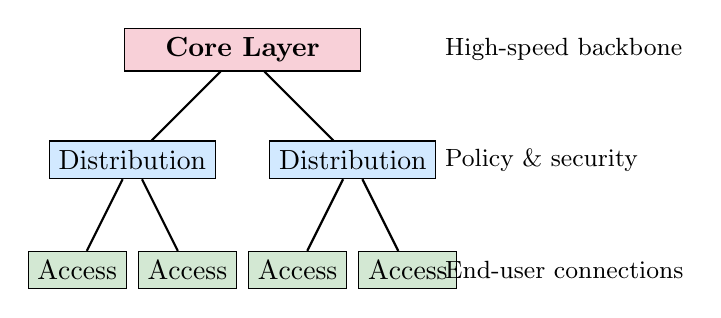
\begin{tikzpicture}[scale=0.7]
				% Core layer
				\node[draw, rectangle, fill=networkred!20, minimum width=3cm] (core) at (0,3) {\textbf{Core Layer}};
				\node[right] at (3.5,3) {\small High-speed backbone};
				
				% Distribution layer
				\node[draw, rectangle, fill=networkblue!20, minimum width=2cm] (dist1) at (-2,1) {Distribution};
				\node[draw, rectangle, fill=networkblue!20, minimum width=2cm] (dist2) at (2,1) {Distribution};
				\node[right] at (3.5,1) {\small Policy \& security};
				
				% Access layer
				\node[draw, rectangle, fill=networkgreen!20] (acc1) at (-3,-1) {Access};
				\node[draw, rectangle, fill=networkgreen!20] (acc2) at (-1,-1) {Access};
				\node[draw, rectangle, fill=networkgreen!20] (acc3) at (1,-1) {Access};
				\node[draw, rectangle, fill=networkgreen!20] (acc4) at (3,-1) {Access};
				\node[right] at (3.5,-1) {\small End-user connections};
				
				% Connections
				\draw[thick] (core) -- (dist1);
				\draw[thick] (core) -- (dist2);
				\draw[thick] (dist1) -- (acc1);
				\draw[thick] (dist1) -- (acc2);
				\draw[thick] (dist2) -- (acc3);
				\draw[thick] (dist2) -- (acc4);
			\end{tikzpicture}
		\end{center}
	\end{frame}
	
	% Slide 28: Collapsed-Core Model - Cost-Effective Design
	\begin{frame}{Collapsed-Core Model - Cost-Effective Design}
		\begin{itemize}
			\item The \textbf{collapsed-core model} combines core and distribution layer functions into a single tier.
			\item This design reduces cost and complexity in small to midsize networks while maintaining functionality.
			\item Modern powerful switching equipment can support both core routing and distribution-layer services effectively.
			\item The collapsed-core still performs the same functions as separate core and distribution layers.
		\end{itemize}
		
		\begin{center}
			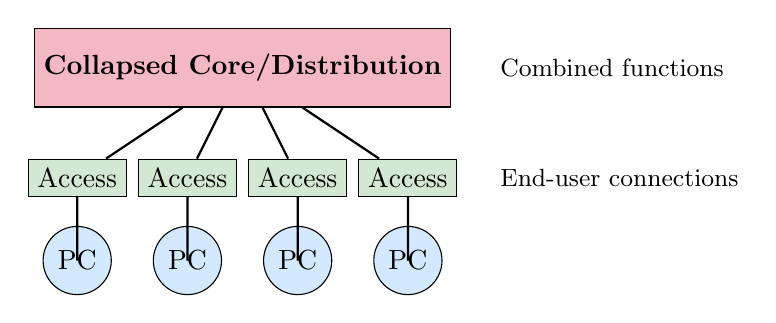
\begin{tikzpicture}[scale=0.7]
				% Collapsed core/distribution layer
				\node[draw, rectangle, fill=networkred!30, minimum width=4cm, minimum height=1cm] (collapsed) at (0,2) {\textbf{Collapsed Core/Distribution}};
				\node[right] at (4.5,2) {\small Combined functions};
				
				% Access layer
				\node[draw, rectangle, fill=networkgreen!20] (acc1) at (-3,0) {Access};
				\node[draw, rectangle, fill=networkgreen!20] (acc2) at (-1,0) {Access};
				\node[draw, rectangle, fill=networkgreen!20] (acc3) at (1,0) {Access};
				\node[draw, rectangle, fill=networkgreen!20] (acc4) at (3,0) {Access};
				\node[right] at (4.5,0) {\small End-user connections};
				
				% End devices
				\node[draw, circle, fill=networkblue!20, minimum size=0.6cm] at (-3,-1.5) {PC};
				\node[draw, circle, fill=networkblue!20, minimum size=0.6cm] at (-1,-1.5) {PC};
				\node[draw, circle, fill=networkblue!20, minimum size=0.6cm] at (1,-1.5) {PC};
				\node[draw, circle, fill=networkblue!20, minimum size=0.6cm] at (3,-1.5) {PC};
				
				% Connections
				\draw[thick] (collapsed) -- (acc1);
				\draw[thick] (collapsed) -- (acc2);
				\draw[thick] (collapsed) -- (acc3);
				\draw[thick] (collapsed) -- (acc4);
				\draw[thick] (acc1) -- (-3,-1.5);
				\draw[thick] (acc2) -- (-1,-1.5);
				\draw[thick] (acc3) -- (1,-1.5);
				\draw[thick] (acc4) -- (3,-1.5);
			\end{tikzpicture}
		\end{center}
	\end{frame}
	
	% Slide 29: Traffic Flow Analysis - North-South vs. East-West
	\begin{frame}{Traffic Flow Analysis - North-South vs. East-West}
		\begin{itemize}
			\item Understanding traffic flow is essential for network security and performance optimization.
			\item \textbf{North-south traffic} flows between your internal network and external Internet connections.
			\item \textbf{East-west traffic} represents lateral movement between servers, data centers, and internal network segments.
			\item Security monitoring must address both traffic types, with increasing focus on east-west due to insider threats.
		\end{itemize}
		
		\begin{center}
			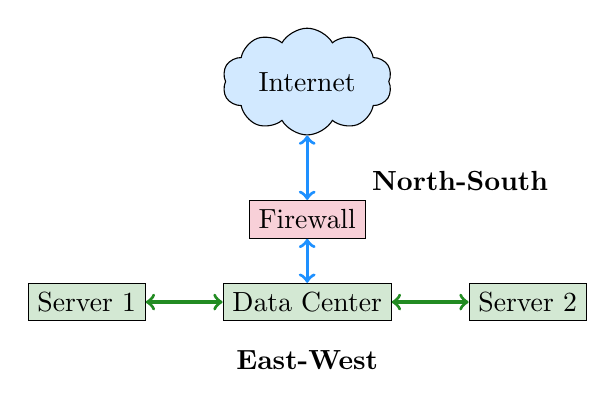
\begin{tikzpicture}[scale=0.7]
				% Internet cloud
				\node[draw, cloud, fill=networkblue!20, cloud puffs=10, cloud puff arc=120, aspect=2, minimum width=2cm, minimum height=1cm] (internet) at (0,4) {Internet};
				
				% Firewall
				\node[draw, rectangle, fill=networkred!20] (firewall) at (0,1.5) {Firewall};
				
				% Internal network
				\node[draw, rectangle, fill=networkgreen!20] (server1) at (-4,0) {Server 1};
				\node[draw, rectangle, fill=networkgreen!20] (server2) at (0,0) {Data Center};
				\node[draw, rectangle, fill=networkgreen!20] (server3) at (4,0) {Server 2};
				
				% North-South arrows
				\draw[very thick, networkblue, <->] (internet) -- (firewall);
				\draw[very thick, networkblue, <->] (firewall) -- (server2);
				\node[right] at (1,2.2) {\textbf{North-South}};
				
				% East-West arrows
				\draw[very thick, networkgreen, <->] (server1) -- (server2);
				\draw[very thick, networkgreen, <->] (server2) -- (server3);
				\node[below] at (0,-0.7) {\textbf{East-West}};
			\end{tikzpicture}
		\end{center}
	\end{frame}
	
	% Slide 30: Virtual Networking and Network Function Virtualization (NFV)
	\begin{frame}{Virtual Networking and Network Function Virtualization (NFV)}
		\begin{itemize}
			\item \textbf{Virtual networking} provides networking services through software rather than dedicated hardware devices.
			\item \textbf{Virtual switches (vSwitch)} operate on hypervisors, eliminating the need for external networking hardware.
			\item \textbf{Virtual Network Interface Cards (vNIC)} connect virtual machines to the hypervisor and network.
			\item \textbf{Network Function Virtualization (NFV)} runs routers, switches, firewalls, and load balancers as software on single devices.
		\end{itemize}
		
		\begin{exampleblock}{Scooby Doo Gang Virtual Network Example}
			Mystery Inc. virtualizes their entire network infrastructure on a single powerful server. Instead of buying separate physical routers, switches, and firewalls, they run virtual versions of each device as software. Fred's virtual machine connects through a vNIC to a virtual switch, which routes traffic through a virtual firewall before reaching Velma's analysis server - all running on the same physical hardware managed by the hypervisor.
		\end{exampleblock}
	\end{frame}
	
	% Slide 31: Chapter Summary and Key Takeaways
	\begin{frame}{Chapter Summary and Key Takeaways}
		\begin{itemize}
			\item Networks enable resource sharing between connected devices using various topologies and architectures.
			\item Physical topologies (bus, star, ring, mesh) each offer distinct advantages and trade-offs for different scenarios.
			\item Network types range from small PANs to global WANs, with specialized networks like SANs for storage.
			\item Modern network design emphasizes virtualization, software-defined approaches, and hierarchical models for scalability.
		\end{itemize}
		
		\begin{block}{Essential Network Concepts}
			\begin{itemize}
				\item \textbf{Fault tolerance} vs. \textbf{cost} considerations in topology selection
				\item \textbf{Centralized} (client-server) vs. \textbf{decentralized} (peer-to-peer) architectures
				\item \textbf{Three-tier model}: Core (backbone), Distribution (policy), Access (end-users)
				\item \textbf{Traffic flow}: North-south (external) and east-west (internal) security implications
			\end{itemize}
		\end{block}
	\end{frame}
	
	% Slide 32: Review Questions and Exam Preparation
	\begin{frame}{Review Questions and Exam Preparation}
		\begin{itemize}
			\item Which topology provides the highest fault tolerance but requires the most connections?
			\item What are the three layers of the hierarchical network model and their primary functions?
			\item How do peer-to-peer and client-server architectures differ in terms of security and scalability?
			\item What is the difference between north-south and east-west traffic flow patterns?
		\end{itemize}
		
		\begin{center}
			\begin{tabular}{ll}
				\toprule
				\textbf{Study Focus Areas} & \textbf{Key Terms} \\
				\midrule
				Network Components & Workstation, Server, Host, Client \\
				Topologies & Bus, Star, Ring, Mesh, Hybrid \\
				Network Types & LAN, WAN, MAN, PAN, CAN, SAN \\
				Architectures & Peer-to-peer, Client-server \\
				Design Models & Three-tier, Collapsed-core, Spine-leaf \\
				Advanced Concepts & MPLS, SDWAN, NFV, Traffic flow \\
				\bottomrule
			\end{tabular}
		\end{center}
	\end{frame}
	
\end{document}